% !TEX TS-program = pdflatex

\documentclass[unicode,11pt,notheorems,xcolor=table]{beamer}

\usepackage[T2A]{fontenc}
\usepackage[utf8]{inputenc}
\usepackage[russian]{babel}
\usepackage{amsmath,amsfonts,amssymb,amsthm}
\usepackage{mathtools}
\usepackage{diagbox}

\usepackage{ulem}
\usepackage{tikz, graphicx}
%\usepackage{tkz-graph}
\usetikzlibrary{matrix,arrows,decorations.pathmorphing, arrows.meta,positioning}
\usetikzlibrary{positioning,calc}
\usetikzlibrary{petri}
\usetikzlibrary{decorations.pathreplacing}

%Описание стиля презентации
\usetheme[sidebar=0]{kfmn} 
\setbeamercovered{transparent}

%\definecolor{cyan}{RGB}{240,217,1}
%\definecolor{vgugreen}{RGB}{143,188,103}
%\definecolor{vgured}{RGB}{234,38,40}
%\definecolor{vgublue}{RGB}{53,101,167}



\makeatletter
	\g@addto@macro{\endtabular}{\rowfont{}}% Clear row font
	\makeatother
	\newcommand{\rowfonttype}{}% Current row font
	\newcommand{\rowfont}[1]{% Set current row font
		\gdef\rowfonttype{#1}#1\ignorespaces%
	}
\makeatother

\newcommand{\myunit}{9mm}
\tikzset{
    node style sp/.style={draw,circle,minimum size=\myunit},
    node style ge/.style={circle,minimum size=\myunit},
    arrow style mul/.style={draw,sloped,midway,fill=white},
    arrow style plus/.style={midway,sloped,fill=white},
}

%[0, 6, 8, 8, 10, 5, 6, 10, 8, 10, 10], 

\pgfdeclareimage[height=8mm]{university-logo}{logo-iem.png}
\logo{\pgfuseimage{university-logo}}
%2[0, 11, 10, 8, 11, 5, 11, 11, 8, 11, 10, 11],

\titlepicture{
	\begin{tikzpicture}[y=1.4cm,overlay,rotate=8]
	\coordinate (O) at (-3cm,0.9cm);
	\filldraw[thick,draw= vgublue, fill=vgublue!20!white] (0,0) circle[radius=4.2cm];
	\clip (0,0) circle[radius=4.2cm];
	\draw (-1.5,1.5) node{
	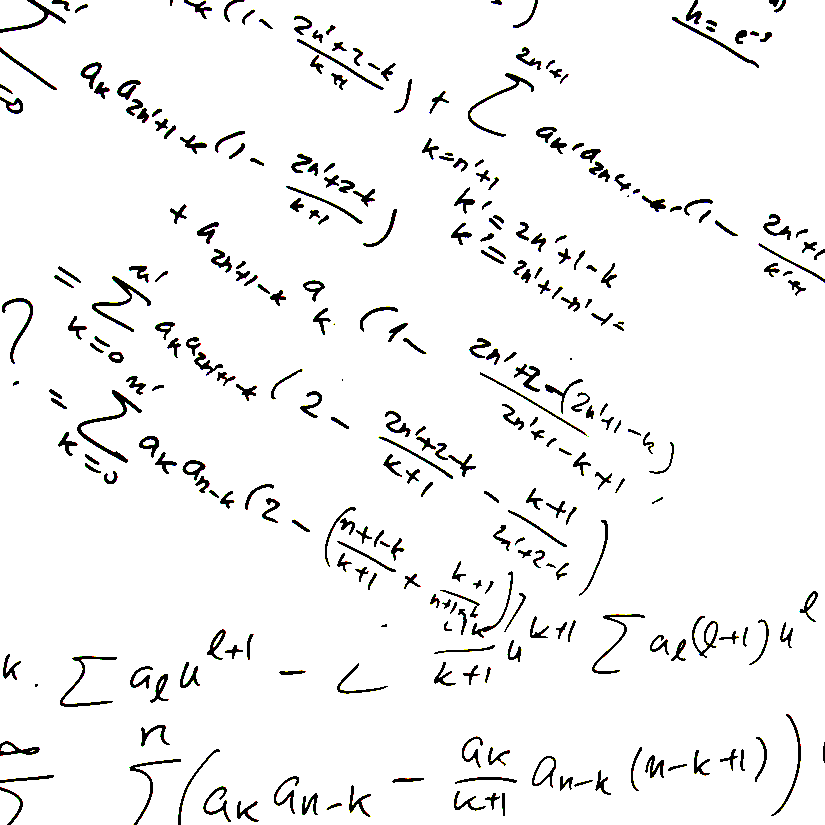
\includegraphics[width=8cm]{titlepic.png}
	};
\end{tikzpicture}
}

\usepackage[math]{iwona}

\newcommand{\hplus}{\mathbin{\hat+}}
\newcommand{\hdot}{\mathbin{\hat\cdot}}
% Описание теорем
\newtheorem{theorem}{Теорема}
\newtheorem{seq}{Следствие}
%%

\LECT % 

% Титульный лист теорем
\author[Д.\,В. Чупраков]{канд.\,физ.-матем.\,наук, доцент Д.\,В. Чупраков\\[6pt] usr10381@vyatsu.ru}

\institute[ВятГУ]{ФГБОУ ВО Вятский государственный университет}

\department{Факультет экономики и финансов}

\title[Лекция~11. Иерархии и приоритеты]{
	Введение в экономико-математическое моделирование\\[12pt]
	Лекция~11. Иерархии и приоритеты}

\date{15 ноября 2020~г.}


\setbeamercovered{invisible}



\begin{document}


\maketitle

\begin{frame}{Структура лекции}
	\tableofcontents
\end{frame}


\begin{frame}{}{}
\begin{itemize}
    \item Метод анализа иерархий (МАИ) разработан американским математиком Томасом Саати. Представляет собой математический инструмент системного подхода к сложным проблемам принятия решений, позволяет комплексно подойти к оценке конкурентоспособности товара, услуги предприятия. 
    \item Метод анализа иерархий широко применяется в сфере управления качеством и конкурентоспособностью
\end{itemize}
\end{frame}



\begin{frame}{Задача принятия решений}{}
    $$
    \alert{X=\{A, K, S, I\}}
    $$
    \begin{itemize}
        \item[$A$~---] множество альтернатив (зависит от имеющейся базы знаний, новизны задачи);
        \item[$K$~---] множество критериев оценки альтернатив (зависит от степени детализации задачи и требуемого качества ее решения);
        \item[$S$~---] метод поиска (вывода) решения:
        \begin{itemize}
            \item способ выбора альтернатив, определяемый структурой предпочтений ЛПР;
            \item метод (модель) оптимизации, обусловливающий способ агрегирования критериев. 
        \end{itemize}
        \item[$I$~---] уровень информации. 
    \end{itemize}
\end{frame}
\begin{frame}{Подход к принятию решений}{}
    \structure{Классический}

    Каждый вариант решения $X$ оценивается неотрицательной  действительно-значной функцией выигрыша g(x).
    $$
        X_\text{опт} =\max g(x). 
    $$
    Применяется в детерминированной среде и условиях риска.

    \medskip
    \structure{Поведенческий}

    Множество последствий каждого варианта $p(x)$ сравнивается с множеством допустимых последствий при решении данной проблемы $p_\text{д}(x)$. 
    Применяется в условиях неопределенности
\end{frame}

\begin{frame}{Классический подход к выбору альтернатив}{}
\begin{itemize}
    \item Метод теории полезности
    \item Метод взвешенной суммы оценок критериев 
    \item Метод анализа иерархий
\end{itemize}
\end{frame}

\begin{frame}[allowframebreaks]{Построение функции полезности}{}
\begin{enumerate}
    \item Провести опрос экспертов.
    \item Построить одномерные функции полезности.
    \item Провести ранжирование возможных исходов без взаимного сравнения альтернатив.
    \item Построить многомерную функцию полезности как аддитивную или мультипликативную комбинацию одномерных функций.
\end{enumerate}

    \bigskip
    \structure{Допущение:} критерии являются взаимно независимыми по полезности. 

    \framebreak
    \bigskip
    \structure{Достоинство:} 
    
    \medskip
    возможность оценки любого количества альтернативных вариантов с использованием полученной функции. 
    
    \bigskip
    \structure{Недостатки:}
    \begin{itemize}
        \item необходимость привлечения значительных объемов информации; 
        \item высокая трудоемкость;
        \item исходная информация должна быть устойчивой. 
    \end{itemize}
    
    
\end{frame}


\begin{frame}[allowframebreaks]{Построение функции полезности}{}
    \begin{enumerate}
        \item Определяется перечень альтернатив и перечень критериев.
        \item Каждой альтернативе дается балльная оценка по каждому из критериев.
        \item Критериям приписываются количественные веса, характеризующие их сравнительную важность. 
        \item Определяется ценность альтернативы путем умножения весов на критериальные оценки с последующим суммированием. 
        \item Выбирается альтернатива с наибольшим показателем ценности. 
    \end{enumerate}
    
    \bigskip
    \structure{Достоинство:} 
    простота и удобство
        
    \bigskip
    \structure{Недостатки:}
    отсутствие научного обоснования при определении весов критериев и альтернатив.                 
\end{frame}
    
\begin{frame}[allowframebreaks]{Метод анализа иерархий}

    \begin{alertblock}{План метода}
    \begin{enumerate}
        \item Декомпозиция проблемы: построение качественной модели проблемы в виде иерархии  включающей 
        \begin{itemize}
            \item цель,
            \item альтернативные варианты достижения цели,
            \item критерии оценки качества альтернатив.
        \end{itemize}
        \item Ранжирование критериев в соответствии с заданной шкалой предпочтений. 
        \begin{itemize}
            \item построение матрицы попарных сравнений,
            \item проверка согласованности,
            \item определение весов критериев.
        \end{itemize}
        \item Вычисление приоритетов по каждой альтернативе.            
        \item Определение оптимальной альтернативы по совокупности критериев.
    \end{enumerate}    
    \end{alertblock}
    \framebreak
    \structure{Достоинства:} 
    \begin{itemize}
        \item метод позволяет найти  вариант, который наилучшим образом согласуется с~пониманием сути проблемы и требованиями к ее решению.
        \item метод позволяет проверить качество субъективных оценок.
    \end{itemize}

    \bigskip
    \structure{Недостатки:}
        Вычислительно сложен.
    
\end{frame}

\section{Метод анализа иерархий}
\subsection{Этап 1. Декомпозиция}

\begin{frame}{Этап 1. Декомпозиция}{}
    \begin{enumerate}
        \item Определение глобальной цели
        \item Определение промежуточных целей (подцелей)
        \item Определение критериев достижимости промежуточных целей 
        \item Формирование альтернатив    
        \item Построение иерархической структуры.
    \end{enumerate}
\end{frame}
\begin{frame}{Иерархическая структура}{}
    \alert{Иерархическая структура}~--- представление проблемы принятия решений в виде графа:
    \begin{itemize}
        \item элементы располагаются по уровням;
        \item на верхнем уровне находится цель принятия решения,
        \item элементы нижнего уровня~--- варианты достижения цели (альтернативы); 
        \item элементы промежуточных уровней~--- критерии или факторам, которые связывают цель с альтернативами;
        \item каждый элемент, за исключением самого верхнего, зависит от одного или более выше расположенных элементов. 
    \end{itemize}
    \begin{block}{Полнота иерархии}
        Иерархия считается \alert{полной}, если любой элемент заданного уровня функционирует как критерий для всех элементов нижестоящего уровня.
    \end{block}
\end{frame}

\begin{frame}{Иерархическая структура}{}
    \centering
    \begin{tikzpicture}[node distance=1.5cm]
        \node[draw,fill=vgured!30] (target) at (4,3) {Цель};

        \node[draw,fill=vgured!30] (subtarget1) at (2,2) {Подцель 1};
        \node[draw,fill=vgured!30] (subtarget2) at (6,2) {Подцель 2};

        \node [draw, align=center] 
            (criteria1) at (0,0) {Критерий 1};
    
        \node [right = of criteria1.center, draw, align=center] 
            (criteria2) {Критерий 2};
    
        \node [right = of criteria2.center, draw, align=center] 
            (criteria3) {Критерий 3};
    
        \node [right = of criteria3.center, draw, align=center] 
            (criteria4) {Критерий 4};
        \node[draw,fill=vgugreen!50]  (alt1) at (0,-4)    {Альтернатива 1};
        \node[draw,fill=vgugreen!50]  (alt2) at (4,-4)  {Альтернатива 2};
        \node[draw,fill=vgugreen!50]  (alt3) at (8.1,-4)    {Альтернатива 3};
    
        \draw 
            (target) 
            edge (subtarget1)
            edge (subtarget2)
        ;

        \draw 
            (subtarget1) 
            edge (criteria1.north)
            edge (criteria2.north)
            edge (criteria3.north)
            % edge (criteria4.north)
        ;
        \draw 
            (subtarget2) 
            % edge (criteria1.north)
            % edge (criteria2.north)
            edge (criteria3.north)
            edge (criteria4.north)
        ;

        \draw 
            (alt1) 
            edge (criteria1.south)
            edge (criteria2.south)
            edge (criteria3.south)
            edge (criteria4.south)
        ;
        \draw 
            (alt2) 
            edge (criteria1.south)
            edge (criteria2.south)
            edge (criteria3.south)
            edge (criteria4.south)
        ;
        \draw 
            (alt3) 
            edge (criteria1.south)
            edge (criteria2.south)
            edge (criteria3.south)
            edge (criteria4.south)
        ;
    \end{tikzpicture}
\end{frame}


\subsection{Этап 2. Ранжирование критериев}
% \begin{frame}{}
    
% \end{frame}

% \begin{frame}{Отношение порядка}{}

% \end{frame}

\begin{frame}{Этап 2. Ранжирование критериев}{}
    \structure{Проблема:} как сравнить критерии между собой.
    \begin{block}{Алгоритм ранжирования критериев}
    \begin{enumerate}
        \item Выбор шкалы ранжирования.
        \item Формирование матрицы попарных сравнений критериев с использованием шкалы предпочтений одного сравниваемого объекта другому.
        \item Вычисление весов критериев и нормализация оценок.
        \item Оценка компонент собственного вектора каждого критерия
        \item Оценка согласованности матрицы
    \end{enumerate}
\end{block}
\end{frame}

\subsection{Ранговая шкала}
\begin{frame}{Раногвая шкала}{}
\begin{block}{Определение}
    Порядковая (ранговая) шкала --- шкала, позволяющая указать последовательность носителей признака по степени выраженности признака. 
\end{block}

\medskip
\alert{Порядковая шкала не позволяет установить как сильно выражен признак у одного носителя по сравнению с другим.}

\structure{Выбор шкалы:}
\begin{itemize}
    \item шкала должна позволять эксперту улавливать разницу в оценках факторов;
    \item эксперт должен быть уверенным во всех градациях своих оценок одновременно.
\end{itemize}
\end{frame}

\begin{frame}{Типовая ранговая шкала}
    \begin{tabular}{cp{9.2cm}}
        \rowcolor{vgublue} \color{white}Ранг & \textcolor{white}{Описание степени превосходства}\tabularnewline
        0 & Объекты не сравнимы \\
        1 & Объекты одинаково важны \\
        3 & Умеренное превосходство одного над другим \\
        5 & Существенное превосходство одного над другим \\
        7 & Значительное превосходство одного над другим \\
        9 & Абсолютное превосходство одного над другим \\
    \end{tabular}

    \bigskip
    \structure{\hrule}
    \bigskip
    % \begin{block}{}
    \begin{itemize}
        \item $a_{ij}>1$ если у носителя~$i$  признак более выражен, чем у~носителя~$j$
        \item $a_{ij}<1$ если у носителя~$j$  признак более выражен, чем у~носителя~$i$.
        \item $a_{ij}= \frac{1}{a_{ji}}$, если признаки сравнимы.
        \item $a_{ij}= a_{ji}=0$, если признаки несравнимы.
    \end{itemize}
    % \end{block}

\end{frame}


\begin{frame}{Матрица попарного сравнения критериев}{}
    \noindent
    \centering
    \begin{tabular}{|>{\columncolor{vgublue!30}\rule[-5mm]{0pt}{12mm}}c|c|c|c|c|c|}
        \hline
        \rowcolor{vgublue!30}Критерии& I& II &  III & $\cdots$ & $n$\\
        \hline
        I & 1 & \cellcolor{yellow!30}$a_{12}$ & \cellcolor{yellow!30} $a_{13}$ &  $\cdots$ & \cellcolor{yellow!30} $a_{1n}$ \\
        \hline
        II & \cellcolor{red!30}  $a_{21}$ & 1 & \cellcolor{yellow!30} $a_{23}$ &$\cdots$ & \cellcolor{yellow!30} $a_{2n}$\\
        \hline
        III & \cellcolor{red!30}  $a_{31}$ & \cellcolor{red!30}  $a_{32}$ & 1 & $\cdots$ & \cellcolor{yellow!30} $a_{3n}$\\
        \hline
        $\cdots$ & $\cdots$ & $\cdots$ & $\cdots$ & $\cdots$ & $\cdots$  \\
        \hline
        $n$ & \cellcolor{red!30} $a_{n1}$ & \cellcolor{red!30} $a_{n2}$ & \cellcolor{red!30} $a_{n3}$ & $\cdots$ & $1$\\
        \hline
    \end{tabular}

    \medskip
    Матрица сравнения критериев \alert{обратно симметричная.}

\end{frame}
\begin{frame}{Вектор приоритетов критериев}

    Ранжирование критериев, анализируемых с помощью , осуществляется на основании главных собственных векторов матрицы парных сравнений.

    \begin{block}{Определение}
        Число $\lambda$ называется \alert{собственным значением}, а ненулевой вектор-столбец $\vec{W}$~--- \alert{собственным вектором} квадратной матрицы $A$, если они связаны соотношением 
        $$
            \alert{A\overrightarrow{W}=\lambda\overrightarrow{W}.}
        $$
    \end{block}

    \bigskip
    Собственный вектор, отвечающий максимальному собственному значению, называется \alert{главным собственным вектором.}
\end{frame}

\begin{frame}{Вычисление собственного вектора}
    Решим уравнение:
    $$
    \alert{A\overrightarrow{W}=\lambda\overrightarrow{W}.}
    $$

    \begin{equation}
        (A-\lambda E)\overrightarrow{W}=0. \tag{$*$}
        \label{eq:1}
    \end{equation}
    
    Это уравнение имеет \alert{ненулевое} решение только в случае, когда 
    \begin{equation}
        \det(A-\lambda E)=0 \tag{$**$}
        \label{eq:2}
    \end{equation}

    \begin{itemize}
        \item Собственные значения квадратной матрицы  могут быть вычислены как решения уравнения~\eqref{eq:2}.
        \item Собственные векторы~--- как решение соответствующих однородных систем~\eqref{eq:1}.
    \end{itemize}
\end{frame}
\begin{frame}[allowframebreaks]{Пример нахождения собственных векторов}
    \begin{exampleblock}{Пример}
        Для матрицы парных сравнений
        $A=\begin{pmatrix}
            1 & 1/4 & 1/2 \\
            4 & 1 & 1/4 \\
            2 & 4  & 1\\
        \end{pmatrix}$
        вычислить главный собственный вектор.
    \end{exampleblock}
    \begin{enumerate}
        \item 
        Составим уравнение $(A-\lambda E)\overrightarrow{W} = 0$
        \begin{gather*}
         \left[ \begin{pmatrix}
            1 & 1/4 & 1/2 \\
            4 & 1 & 1/4 \\
            2 & 4  & 1\\
        \end{pmatrix} 
        - \lambda \begin{pmatrix}
            1 & 0 & 0 \\
            0 & 1 & 0 \\
            0 & 0  & 1\\
        \end{pmatrix}
        \right] \overrightarrow{W} = 0\\
        \alert{\begin{pmatrix}
               1-\lambda & 1/4 & 1/2 \\
               4 & 1-\lambda & 1/4 \\
               2 & 4  & 1-\lambda\\
           \end{pmatrix} 
        \overrightarrow{W} = 0}
        \end{gather*}
    \item 
    Приравняем определитель к нулю:
    \begin{multline*}
     \det(A-\lambda E)
     = \begin{vmatrix}
           1-\lambda & 1/4 & 1/2 \\
           4 & 1-\lambda & 1/4 \\
           2 & 4  & 1-\lambda\\
       \end{vmatrix} 
       =\\
       = -\frac{1}{8} (2\lambda-7)(4{\lambda^2} + 2\lambda+7)
       =0
    \end{multline*}
    \item Решая это уравнение получаем $\lambda =\frac{7}{2}=3.5$ Это единственный действительной корень уравнения.
    
    \framebreak
    \item Теперь подставим найденное собственное значение в~уравнение $(A-\lambda E)\overrightarrow{W} = 0$
    $$
    \begin{pmatrix}
        1-\frac{7}{2}& 1/4 & 1/2 \\
        4 & 1-\frac{7}{2} & 1/4 \\
        2 & 4  & 1-\frac{7}{2}\\
    \end{pmatrix} 
    \begin{pmatrix}
        w_1 \\ w_2 \\ w_3
    \end{pmatrix} 
    = 
    \begin{pmatrix}
        0 \\ 0 \\ 0
    \end{pmatrix}     
    $$
    $$
    \begin{pmatrix}
        -\frac{5}{2}& 1/4 & 1/2 \\
        4 & -\frac{5}{2} & 1/4 \\
        2 & 4  & -\frac{5}{2}\\
    \end{pmatrix} 
    \begin{pmatrix}
        w_1 \\ w_2 \\ w_3
    \end{pmatrix} 
    = 
    \begin{pmatrix}
        0 \\ 0 \\ 0
    \end{pmatrix}     
    $$    
    \alert{$$
    \left\lbrace
    \begin{aligned}
        -\frac{5}{2}w_1+ \frac{1}{4}w_2 + \frac{1}{2}w_3 &= 0 \\
        4w_1 -\frac{5}{2}w_2 +  \frac{1}{4}w_3 &= 0 \\
        2w_1 + 4w_2 -\frac{5}{2}w_3 &= 0\\
    \end{aligned}
    \right.
    $$}
    \framebreak 
    \item Решая систему получим множество собственных векторов:
    $$
    \left\lbrace
    \begin{aligned}
        w_1 &= \frac{1}{4}\alpha\\
        w_2 &= \frac{1}{2}\alpha\\
        w_3 &= \alpha\\
    \end{aligned}
    \right.
    $$
    \item Вычислим нормированный вектор~--- вектор сумма координат которого равна 1: 
    $$
        \frac{1}{4}\alpha+\frac{1}{2}\alpha + \alpha= \alpha \frac{7}{4}=1
    $$
    \item Подставляя $\alpha=\frac{4}{7}$ получаем.
        $$
            \alert{\overrightarrow{W}_{\lambda_{\max} }=(w_1,w_2,w_3) = \left( \frac{1}{7}, \frac{2}{7},\frac{4}{7} \right)}
        $$
\end{enumerate}
\framebreak

Итак,  
$$
    \frac{1}{7} < \frac{2}{7} < \frac{4}{7},
$$
$$
    w_1< w_2 < w_3.
$$

\bigskip
Третья альтернатива наиболее предпочтительная, затем идет вторая и первая.
\end{frame}

\begin{frame}[allowframebreaks]{Вычисление весов критериев}
    Для обратно симметричной матрицы есть более простой алгоритм.

    \begin{block}{Алгоритм}
    \begin{enumerate}
        \item Перемножить  все  элементы  каждой  строки и извлечь    корень $n$-й степени,  где $n$~--- число элементов  в  строке:
        $$
            \alert{ y_i = \sqrt[n]{ \prod_{j=1}^n a_{ij} } }
        $$
        \item Нормировать  их  так,  чтобы  их  сумма  равнялась  единице: 
        $$
            \alert{ y_{i\text{н}} = \frac{y_i}{ \sum_{j=1}^n y_{j} } }
        $$
    \end{enumerate}
    \end{block}
    \framebreak
    \begin{itemize}
        \item Вектор $( y_{1\text{н}},\ldots,y_{n\text{н}} )$~--- это  главный собственный вектор $\overrightarrow{W}_{\lambda_{\max} }$.
        \item Величина $y_{i\text{н}} $~--- вклад критерия $A_i$ в достижение цели.
    \end{itemize}

    \structure{Пример:}
    $$
    A=\begin{pmatrix}
        1 & 1/4 & 1/2 \\
        4 & 1 & 1/4 \\
        2 & 4  & 1\\
    \end{pmatrix}
    \to
    \overrightarrow{W}_{\lambda_{\max} }=\begin{pmatrix}
        \sqrt[3]{1\cdot 1/4\cdot 1/2} \\
        \sqrt[3]{4 \cdot 1 \cdot 1/4} \\
        \sqrt[3]{2 \cdot  4 \cdot 1}\\
    \end{pmatrix}
    =
    \begin{pmatrix}
        1/2 \\
        1\\
        2\\
    \end{pmatrix}    
    $$
    $$
        \alert{\overrightarrow{W}_{\lambda_{\max} }}
        = \frac{\vec{w}}{|\vec{w}|} 
        = \frac{1}{1/2+1+2}\left(\frac{1}{2},1,2\right)
        = \alert{\left( \frac{1}{7}, \frac{2}{7},\frac{4}{7}\right)}
    $$
\end{frame}

\begin{frame}[allowframebreaks]{Согласованность матрицы}{}
    \structure{Как хорошо мы построили матрицу попарных оценок?}
    \begin{itemize}
        \item Если $A_i$ предпочтительнее $A_j$, а $A_j$ предпочтительнее $A_k$, то $A_i$ предпочтительней $A_k$
        \item Чем длиннее цепочка предпочтительности
        $$
            A_i \prec A_{j_1} \prec A_{j_2}\ldots \prec A_{j_t} \prec A_{k}
        $$
        между $A_i$ и $A_k$, тем существеннее выражен признак у объекта $A_k$, чем у~$A_i$.
    \end{itemize}

    \begin{block}{Определение}
        \alert{Полная согласованность} матрицы~--- выполнение двух свойств:
        \begin{itemize}
            \item $A_i\prec A_j$, а $A_j \prec A_k$, то $A_i \prec A_k$.
            \item $\alert{a_{ij}a_{jk}=a_{ik}.}$
        \end{itemize}
    \end{block}
    \framebreak
        \begin{itemize}
            \item Если матрица $A$ полностью согласована, то достаточно знать одну ее строку, чтобы вычислить все остальные. 
            \item Полная согласованность обратно симметричной матрицы $n\times n$ эквивалентна требованию равенства 
            $$
               \alert{\lambda_{\max} =n }
            $$
            \item Если предпочтительность объектов оценена только по шкале Саати, то полная согласованность  не достижима.
        \end{itemize}
    \end{frame}
    \begin{frame}{Показатели согласованности}
    \begin{itemize}
        \item Максимальное собственное значение: 
        $$
           \Lambda = \begin{pmatrix}
               \Lambda_1\\ \Lambda_2\\ \cdots \\ \Lambda_n 
           \end{pmatrix} = A\cdot \overrightarrow{W}_{\lambda_{\max} },
            \qquad
            \alert{\lambda_{\max} = \sum_{i=1}^n \Lambda_i}          
        $$
        \item Индекс согласованности:
        $\alert{ \text{ИС}= \dfrac{\lambda_{\max}-n}{n-1} }$

        \medskip
        \item Случайная согласованность:
        
        \begin{tabular}{|>{\columncolor{vgublue!30}}c|c|c|c|c|c|c|c|c|c|c|}
            \hline
            $n$ & 1 & 2 & 3& 4& 5& 6& 7& 8 & 9 & 10\\
            \hline
            СС & 0 & 0 & 0.58 & 0.9& 1.12& 1.24& 1.32& 1.41 & 1.45 & 1.49\\
            \hline 
        \end{tabular}
        \medskip
        \item Отношение согласованности:
        $\alert{\text{ОС}= \dfrac{\text{ИС}}{\text{СС}}}  $
    \end{itemize}
\end{frame}
\begin{frame}{Определение согласованности матирцы}
    \begin{itemize}
        \item \alert{$\text{ОС} \leqslant 0.1$}~--- матрица согласована 
        \item \alert{$0.1 < \text{ОС} \leqslant 0.2$}~--- согласованность матрицы приемлема 
        \item \alert{$\text{ОС}>0.2$}~--- согласованность матрицы неприемлема 
    \end{itemize}
\end{frame}
\begin{frame}[allowframebreaks]{Пример. Cогласованность матирцы}
    \begin{exampleblock}{}
        Проверим согласованность матрицы  
        $A=\begin{pmatrix}
            1 & 1/4 & 1/2 \\
            4 & 1 & 1/4 \\
            2 & 4  & 1\\
        \end{pmatrix}$ 
    \end{exampleblock}
    \begin{itemize}
        \item Мы помним, что 
        \alert{$\overrightarrow{W}_{\lambda_{\max} }
        = \left( \frac{1}{7}, \frac{2}{7},\frac{4}{7}\right)
        $}
        \item Умножим матрицу $A$ на $\overrightarrow{W}_{\lambda_{\max} }$
        $$
           \alert{ \Lambda = A \cdot \overrightarrow{W}_{\lambda_{\max} } =
            \begin{pmatrix}
                1 & 1/4 & 1/2 \\
                4 & 1 & 1/4 \\
                2 & 4  & 1\\
            \end{pmatrix}
            \begin{pmatrix}
                1/7\\
                2/7\\
                4/7\\
            \end{pmatrix}
            = 
            \begin{pmatrix}
                1/2\\
                1\\
                2\\
            \end{pmatrix}
           }
            $$
        \item Сложим координаты вектора: \alert{$\lambda_{\max}= \frac{1}{2}+1+2 = \frac{7}{2}$}
        \framebreak
        \item Вычислим индекс согласованности  
        $$
        \alert{\text{ИС}= \dfrac{\lambda_{\max}-n}{n-1} = \dfrac{7/2-3}{3-1}=\frac{1}{4}=0.25}
        $$
        \item По таблице найдем индекс случайной согласованности 
        \alert{$\text{CС}= 0.58$}
        \item Вычислим отношение согласованности
        $\alert{\text{ОС}= \dfrac{\text{ИС}}{\text{СС}}} =\frac{0.25}{0.58} \approx 0.43$
        \item  Так как \alert{$\text{ОС}=0.43>0.2$} матрица не согласована.
    \end{itemize}
    
    \bigskip
    \hrule

    \bigskip
    Итак, матрица  $A=\begin{pmatrix}
        1 & 1/4 & 1/2 \\
        4 & 1 & 1/4 \\
        2 & 4  & 1\\
    \end{pmatrix}$  не согласована.
\end{frame}

\subsection{Этап 3. Приоритеты альтернатив по критериям}
\begin{frame}{Этап 3. Приоритеты альтернатив по критериям}
    \begin{itemize}
        \item Альтернативы сравниваются попарно с целью получения локальных векторов приоритета по каждому критерию.
        \item Строится матрица попарных сравнений $x_{ij}$ альтернатив~$i$ и~$j$ по  критерию $A_k$. (Помним, что $x_{ij}=\frac{1}{x_{ji}}$).
        \item По построенной матрице вычисляется нормализованный вектор приоритетов по рассмотренной методике.
    \end{itemize}
    В результате получается вектор 
    $$
    \alert{
    X^{(k)} = \begin{pmatrix}
        X^{(k)}_{1\text{н}}\\ X^{(k)}_{2\text{н}}\\ \cdots \\ X^{(k)}_{m\text{н}}
    \end{pmatrix}
    }
    $$

\end{frame}

\begin{frame}{Матрица попарного сравнения альтернатив}{}
    \noindent
    \centering
    \begin{tabular}{|>{\columncolor{vgublue!30}\rule[-5mm]{0pt}{12mm}}c|c|c|c|c|c|}
        \hline
        \rowcolor{vgublue!30}Альтернативы& I& II &  III & $\cdots$ & $m$\\
        \hline
        I & 1 & \cellcolor{yellow!30}$x_{12}$ & \cellcolor{yellow!30} $x_{13}$ &  $\cdots$ & \cellcolor{yellow!30} $x_{1m}$ \\
        \hline
        II & \cellcolor{red!30}  $x_{21}$ & 1 & \cellcolor{yellow!30} $x_{23}$ &$\cdots$ & \cellcolor{yellow!30} $x_{2m}$\\
        \hline
        III & \cellcolor{red!30}  $x_{31}$ & \cellcolor{red!30}  $x_{32}$ & 1 & $\cdots$ & \cellcolor{yellow!30} $x_{3m}$\\
        \hline
        $\cdots$ & $\cdots$ & $\cdots$ & $\cdots$ & $\cdots$ & $\cdots$  \\
        \hline
        $m$ & \cellcolor{red!30} $x_{m1}$ & \cellcolor{red!30} $x_{m2}$ & \cellcolor{red!30} $x_{m3}$ & $\cdots$ & $1$\\
        \hline
    \end{tabular}    
\end{frame}

\subsection{Этап 4. Приоритет альтернатив}
\begin{frame}{Этап 4. Приоритет альтернатив}{}
    {
    \noindent
    \centering
    \begin{tabular}{|>{\columncolor{vgured!30}\rule[-2mm]{0pt}{7mm}}p{3.5cm}|c|c|c|c|c|>{\columncolor{vgured!30}}c|}
        \hline
        \rowcolor{vgublue!30}Критерии& $A_1$& $A_2$ &  $A_3$ & $\cdots$ & $A_n$ & Оценка\\
        \hline
        \rowcolor{vgugreen!30}Приоритет критерия& $y_{1\text{н}}$& $y_{2\text{н}}$ &  $y_{3\text{н}}$ & $\cdots$ & $y_{n\text{н}}$ & \\
        \hline
        Альтернатива I & $X^{(1)}_{1\text{н}}$ & $X^{(2)}_{1\text{н}}$ & $X^{(3)}_{1\text{н}}$ &  $\cdots$ & $X^{(n)}_{1\text{н}}$ & $A_1$\\
        \hline
        Альтернатива II & $X^{(1)}_{2\text{н}}$ & $X^{(2)}_{2\text{н}}$ & $X^{(3)}_{2\text{н}}$ &  $\cdots$ & $X^{(n)}_{2\text{н}}$ & $A_2$\\
        \hline
        Альтернатива III & $X^{(1)}_{3\text{н}}$ & $X^{(2)}_{3\text{н}}$ & $X^{(3)}_{3\text{н}}$ &  $\cdots$ & $X^{(n)}_{3\text{н}}$ & $A_3$\\        
        \hline
        $\cdots$ & $\cdots$ & $\cdots$ & $\cdots$ & $\cdots$ & $\cdots$  & $\cdots$ \\
        \hline
        Альтернатива $m$ & $X^{(1)}_{m\text{н}}$ & $X^{(2)}_{m\text{н}}$ & $X^{(3)}_{m\text{н}}$ &  $\cdots$ & $X^{(n)}_{3\text{н}}$ & $A_m$\\        
        \hline
    \end{tabular}   
    \par}
    \bigskip
    Оценка альтернативы $i$ вычисляется как скалярное произведение строки ,,\structure{Приоритет критерия}`` на строку ,,\structure{Альтернатива $i$}``:
    $$
        \alert{A_i= \sum_{j=1}^n X^{(j)}_{i\text{н}}}
    $$
\end{frame}

\section{Пример }
\begin{frame}{Пример}

\begin{tabular}{|>{\columncolor{vgublue!20}}p{4cm}|c|c|c|}
    \hline
    \rowcolor{vgublue!20}& Проект 1 & Проект 2 & Проект 3\\
    \hline
    Вложения (млн. руб) & 5 & 5.5 & 4.5 \\
    \hline
    Срок реализации (лет) & 3 & 2 & 3 \\
    \hline
    Кол-во рабочих мест & 20 & 5 & 0 \\
    \hline
    Качество документации & среднее & низкое & высокое \\
    \hline
\end{tabular}

\end{frame}


\begin{frame}{Этап декомпозиции}{}
\centering
    \begin{tikzpicture}[node distance=1.5cm]
        \node[draw,fill=vgured!30] (target) at (4,3) {Проект для реализации};

        \node [draw, align=center] 
            (criteria1) at (0,0) {Вложения\\{\phantom{р}}};

        \node [right = of criteria1.center, draw, align=center] 
            (criteria2) {Срок\\ реализации};

        \node [right = of criteria2.center, draw, align=center] 
            (criteria3) {Количество\\ рабочих мест};

        \node [right = of criteria3.center, draw, align=center] 
            (criteria4) {Качество\\ документации};
        \node[draw,fill=vgugreen!50]  (alt1) at (0,-4)    {Проект 1};
        \node[draw,fill=vgugreen!50]  (alt2) at (4,-4)  {Проект 2};
        \node[draw,fill=vgugreen!50]  (alt3) at (8.1,-4)    {Проект 3};

        \draw 
            (target) 
            edge (criteria1.north)
            edge (criteria2.north)
            edge (criteria3.north)
            edge (criteria4.north)
        ;

        \draw 
            (alt1) 
            edge (criteria1.south)
            edge (criteria2.south)
            edge (criteria3.south)
            edge (criteria4.south)
        ;
        \draw 
            (alt2) 
            edge (criteria1.south)
            edge (criteria2.south)
            edge (criteria3.south)
            edge (criteria4.south)
        ;
        \draw 
            (alt3) 
            edge (criteria1.south)
            edge (criteria2.south)
            edge (criteria3.south)
            edge (criteria4.south)
        ;
    \end{tikzpicture}
\end{frame}
\begin{frame}{Ранжирование критериев}{}
    \small
        \begin{tabular}{|>{\columncolor{vgublue!20}}p{1.5cm}|>{\centering}p{1.5cm}|>{\centering}p{1.5cm}|>{\centering}p{1.5cm}|>{\centering}p{1.5cm}|>{\centering}p{1.5cm}|}
            \hline
            \rowcolor{vgublue!20}& Вложения & Срок реализации & Кол-во рабочих мест & Качество документации\tabularnewline
            \hline
            Вложения  & \visible<1->{$1$} & \cellcolor{yellow!40} \visible<2->{$3$} & \cellcolor{yellow!40} \visible<2->{$5$} & \cellcolor{yellow!40} \visible<2->{$9$} \tabularnewline
            \hline
            Срок реализации& \cellcolor{red!20} \visible<3->{$\dfrac{1}{3}$} & \visible<1->{$1$} & \cellcolor{yellow!40} \visible<2->{$3$} & \cellcolor{yellow!40} \visible<2->{$5$}\tabularnewline
            \hline
            Кол-во рабочих мест &   \cellcolor{red!20} \visible<3->{$\dfrac{1}{5}$}&  \cellcolor{red!20}  \visible<3->{$\dfrac{1}{3}$} & \visible<1->{$1$}  & \cellcolor{yellow!40} \visible<2->{$7$}\tabularnewline
            \hline
            Качество документации & \cellcolor{red!20} \visible<3->{$\dfrac{1}{9}$} &\cellcolor{red!20} \visible<3->{$\dfrac{1}{5}$}  &\cellcolor{red!20} \visible<3->{$\dfrac{1}{7}$} & \visible<1->{$1$} \tabularnewline
            \hline
        \end{tabular}
\end{frame}

\begin{frame}[allowframebreaks]{Пример. Вычисление весов критериев}
    \small
    \begin{tabular}{|>{\columncolor{vgublue!20}}p{1.2cm}|>{\centering}p{1.2cm}|>{\centering}p{1.2cm}|>{\centering}p{1.2cm}|>{\centering}p{1.2cm}|>{\centering\columncolor{vgugreen!30}}p{2cm}|}
        \hline
        \rowcolor{vgublue!20}& Вложения & Срок реализации & Кол-во рабочих мест & Качество документации & $y_i$  \tabularnewline
        \hline
        Вложения  & $1$ & $3$ & $5$ & $9$ & $\sqrt[4]{3\cdot 5\cdot 9} \approx 3.41$  \tabularnewline
        \hline
        Срок реализации& $1/3$ & $1$ & $3$ & $5$ & $\sqrt[4]{\frac{1}{3}\cdot 3 \cdot 5} \approx 1.50$\tabularnewline
        \hline
        Кол-во рабочих мест & $1/5$ & $1/3$ & $1$  & $7$ & $\sqrt[4]{\frac{1}{5}\cdot \frac{1}{3} \cdot 7} \approx 0.83$ \tabularnewline
        \hline
        Качество документации & $1/9$ & $1/5$  & $1/7$ & $1$ & $\sqrt[4]{\frac{1}{9}\cdot \frac{1}{5} \cdot \frac{1}{7}} \approx 0.24$ \tabularnewline
        \hline
    \end{tabular}
    \framebreak
    $$
    W= 
    \frac{1}{3.41+1.50+0.83+0.24}
    \begin{pmatrix}
        3.41 \\ 1.50\\ 0.83\\0.24
    \end{pmatrix}
    =
    \begin{pmatrix}
        0.57 \\ 0.25 \\ 0.14 \\ 0.04
    \end{pmatrix}
    $$

    \bigskip
    \structure{Согласованность}
    \begin{itemize}
    \item Умножим матрицу $A$ на $\overrightarrow{W}_{\lambda_{\max} }$
    $$
       \alert{ \Lambda = A \cdot \overrightarrow{W}_{\lambda_{\max} } =
        \begin{pmatrix}
            1 & 3 & 5 & 9 \\
            1/3 & 1 & 3 & 5\\
            1/5 & 1/3  & 1 & 7\\
            1/9 & 1/5 & 1/78 & 1
        \end{pmatrix}
        \begin{pmatrix}
           0.57\\
            0.25\\
            0.14\\
            0.04
        \end{pmatrix}
        = 
        \begin{pmatrix}
            2.38\\
            1.06\\
            0.62\\
            0.17
        \end{pmatrix}
       }
        $$
    \item Сложим координаты вектора: \alert{$\lambda_{\max}= 4.23$}
    \framebreak
    \item Вычислим индекс согласованности  
    $$
    \alert{\text{ИС}= \dfrac{\lambda_{\max}-n}{n-1} = \dfrac{4.23-4}{4-1}=0.077}
    $$
    \item По таблице найдем индекс случайной согласованности 
    \alert{$\text{CС}= 0.9$}
    \item Вычислим отношение согласованности
    $\alert{\text{ОС}= \dfrac{\text{ИС}}{\text{СС}}} =\frac{0.077}{0.9} \approx 0.09<0.1$
    \item  Матрица согласована.    
    \end{itemize}
    Итак, веса критериев
    
    \begin{tabular}{|p{1.6cm}|p{1.6cm}|p{1.6cm}|p{1.6cm}|p{1.6cm}|}
        \hline
        Критерий & Вложения & Срок реализации & Кол-во рабочих мест & Качество документации \\
        \hline
        Приоритет критерия  & $2.38$ & $1.06$ & $0.62$ & $0.017$ \\
        \hline
    \end{tabular}
\end{frame}

\begin{frame}{Требуемые вложения}
    \begin{tabular}{c|ccc|cc}
    \hline
        Альтернативы & Проект 1 & Проект 2 & Проект 3 & $y_i$ & $y_{i\text{н}}$\\
    \hline
        Проект 1 & 1 & 7 & 9 & 1 & 0.258\\
        Проект 2 & 1/7 & 1  & 3 & 0.405 & 0.105\\
        Проект 3 & 1/9 & 1/3  & 1 & 2.466 & 0.637\\
    \hline
        Сумма & & & & 3.872 & 1\\
    \hline
    \end{tabular}
    \structure{Согласованность.}
    $$
    \text{ИС}=0.019\qquad \text{CC}= 0.58,\qquad \text{ОС}=0.033
    $$
\end{frame}

\begin{frame}{Сроки реализации}
    \begin{tabular}{c|ccc|cc}
    \hline
        Альтернативы & Проект 1 & Проект 2 & Проект 3 & $y_i$ & $y_{i\text{н}}$\\
    \hline
        Проект 1 & 1 & 1/5 & 1 & 0.585 & 0.143\\
        Проект 2 & 5 & 1  & 5 & 2.924 & 0.714\\
        Проект 3 & 7 & 1/5  & 1 & 0.585 & 0.143\\
    \hline
        Сумма & & & & 4.094 & 1\\
    \hline
    \end{tabular}
    \structure{Согласованность.}
    $$
    \text{ИС}=0\qquad \text{CC}= 0.58,\qquad \text{ОС}=0
    $$
\end{frame}
\begin{frame}{Количество рабочих мест}
    \begin{tabular}{c|ccc|cc}
    \hline
        Альтернативы & Проект 1 & Проект 2 & Проект 3 & $y_i$ & $y_{i\text{н}}$\\
    \hline
        Проект 1 & 1 & 7 & 9 & 3.979 & 0.785\\
        Проект 2 & 1/7 & 1  & 3 & 0.754 & 0.149\\
        Проект 3 & 1/9 & 1/3  & 1 & 0.333 & 0.066\\
    \hline
        Сумма & & & & 5.066 & 1\\
    \hline
    \end{tabular}
    % \structure{Согласованность.}
    % $$
    % \text{ИС}=0\qquad \text{CC}= 0.58,\qquad \text{ОС}=0
    % $$
\end{frame}
\begin{frame}{Качество документации}
    \begin{tabular}{c|ccc|cc}
    \hline
        Альтернативы & Проект 1 & Проект 2 & Проект 3 & $y_i$ & $y_{i\text{н}}$\\
    \hline
        Проект 1 & 1 & 1/3 & 3 & 1 & 0.258\\
        Проект 2 & 3 & 1  & 5 & 2.466 & 0.637\\
        Проект 3 & 1/3 & 1/5  & 1 & 0.405 & 0.105\\
    \hline
        Сумма & & & & 3.871 & 1\\
    \hline
    \end{tabular}
    % \structure{Согласованность.}
    % $$
    % \text{ИС}=0\qquad \text{CC}= 0.58,\qquad \text{ОС}=0
    % $$
\end{frame}


\begin{frame}{Приоритет альтернатив}{}
    {
    \noindent
    \centering
    \begin{tabular}{|>{\columncolor{vgured!30}\rule[-2mm]{0pt}{7mm}}p{3.5cm}|c|c|c|c|>{\columncolor{vgured!30}}c|}
        \hline
        \rowcolor{vgublue!30}Критерии& $A_1$& $A_2$ &  $A_3$ & $A_4$ &  Оценка\\
        \hline
        \rowcolor{vgugreen!30}Приоритет критерия& $2.38$& $1.06$ &  $0.62$ & $0.02$ &  \\
        \hline
        Проект 1 & $0.258$ & $0.143$ & $0.785$ &   $0.258$ & $0.30$\\
        \hline
        Проект 2 & $0.105$ & $0.714$ & $0.149$ &  $0.637$ & $0.29$\\
        \hline
        Проект 3 & $0.637$ & $0.143$ & $0.066$ &  $0.105$ & \cellcolor{yellow!50} $0.41$\\        
        \hline
    \end{tabular}   
    \par}
    \vspace{3cm}
    Итак, для нас оптимален проект 3.
\end{frame}
% \section{Резюме и источники}
% \begin{frame}{Резюме}
% 	Теперь вы знаете:
% 	\begin{enumerate}
% 	\item 
% 		Понятие многокритериальной задачи.
% 	\item 
% 		Понятие границы Парето.
%     \item 
% 		Метод идеальной точки.
% 	\end{enumerate}
	
% 	Вы должны уметь:
% 	\begin{itemize}
% 		\item 
% 			Применять метод сетки для приближенного нахождения границы Парето.
% 		\item 
% 			Приводить многокритериальную задачу к каноническому виду.
% 		\item 
% 			Решать многокритериальные задачи линейного программирования методом идеальной точки.
% 	\end{itemize}
	
% \end{frame}
% % \begin{frame}{Литература}
% % \begin{itemize}
% %     \item \href{https://ru.wikipedia.org/wiki/%D0%9C%D0%B5%D1%82%D0%BE%D0%B4_%D0%B0%D0%BD%D0%B0%D0%BB%D0%B8%D0%B7%D0%B0_%D0%B8%D0%B5%D1%80%D0%B0%D1%80%D1%85%D0%B8%D0%B9}{Википедия. Метод анализа иерархий} 
% %     \item 
% %     	Все материалы по курсу здесь:
% %         {\color{blue}\url{https://cloud.mail.ru/public/48BX/47oESuaQQ}}
% % \end{itemize}
% % \end{frame}

\end{document}
